% Options for packages loaded elsewhere
\PassOptionsToPackage{unicode}{hyperref}
\PassOptionsToPackage{hyphens}{url}
%
\documentclass[
]{article}
\usepackage{amsmath,amssymb}
\usepackage{lmodern}
\usepackage{iftex}
\ifPDFTeX
  \usepackage[T1]{fontenc}
  \usepackage[utf8]{inputenc}
  \usepackage{textcomp} % provide euro and other symbols
\else % if luatex or xetex
  \usepackage{unicode-math}
  \defaultfontfeatures{Scale=MatchLowercase}
  \defaultfontfeatures[\rmfamily]{Ligatures=TeX,Scale=1}
\fi
% Use upquote if available, for straight quotes in verbatim environments
\IfFileExists{upquote.sty}{\usepackage{upquote}}{}
\IfFileExists{microtype.sty}{% use microtype if available
  \usepackage[]{microtype}
  \UseMicrotypeSet[protrusion]{basicmath} % disable protrusion for tt fonts
}{}
\makeatletter
\@ifundefined{KOMAClassName}{% if non-KOMA class
  \IfFileExists{parskip.sty}{%
    \usepackage{parskip}
  }{% else
    \setlength{\parindent}{0pt}
    \setlength{\parskip}{6pt plus 2pt minus 1pt}}
}{% if KOMA class
  \KOMAoptions{parskip=half}}
\makeatother
\usepackage{xcolor}
\usepackage{graphicx}
\makeatletter
\def\maxwidth{\ifdim\Gin@nat@width>\linewidth\linewidth\else\Gin@nat@width\fi}
\def\maxheight{\ifdim\Gin@nat@height>\textheight\textheight\else\Gin@nat@height\fi}
\makeatother
% Scale images if necessary, so that they will not overflow the page
% margins by default, and it is still possible to overwrite the defaults
% using explicit options in \includegraphics[width, height, ...]{}
\setkeys{Gin}{width=\maxwidth,height=\maxheight,keepaspectratio}
% Set default figure placement to htbp
\makeatletter
\def\fps@figure{htbp}
\makeatother
\setlength{\emergencystretch}{3em} % prevent overfull lines
\providecommand{\tightlist}{%
  \setlength{\itemsep}{0pt}\setlength{\parskip}{0pt}}
\setcounter{secnumdepth}{-\maxdimen} % remove section numbering
\ifLuaTeX
  \usepackage{selnolig}  % disable illegal ligatures
\fi
\IfFileExists{bookmark.sty}{\usepackage{bookmark}}{\usepackage{hyperref}}
\IfFileExists{xurl.sty}{\usepackage{xurl}}{} % add URL line breaks if available
\urlstyle{same} % disable monospaced font for URLs
\hypersetup{
  pdftitle={A Branch-and-Regret Heuristic for Stochastic and Dynamic Vehicle Routing Problems},
  hidelinks,
  pdfcreator={LaTeX via pandoc}}

\title{A Branch-and-Regret Heuristic for Stochastic and Dynamic Vehicle
Routing Problems}
\author{Lorenzo Sciandra}
\date{giugno 2022}

\begin{document}
\maketitle

\emph{Authors: L. M. Hvattum, A. Lokketangen}\\
\emph{Year: 2007}

\hypertarget{descrizione-del-problema}{%
\section{Descrizione del Problema}\label{descrizione-del-problema}}

\hypertarget{mathbfvrp-stocastico-e-dinamico}{%
\subsection{\texorpdfstring{VRP Stocastico e
Dinamico}{VRP Stocastico e Dinamico}}\label{mathbfvrp-stocastico-e-dinamico}}

Il problema è basato su un caso reale che interessa una delle più grandi
compagnie di distribuzioni in Norvegia. Uno dei servizi che offrono
infatti riguarda il ritiro di beni dai clienti per portarli ad un
deposito centrale dal quale verranno successivamente spediti ovunque. I
clienti possono chiamare per il servizio in qualsiasi momento e la loro
richiesta deve essere \textbf{gestita entro il giorno in questione}.
Solo la metà circa degli ordini serviti ogni giorno sono però
conosciuti all'inizio del giorno lavorativo, l'altra \textbf{metà sono
dinamici}. Nello specifico ogni cliente ha a disposizione delle
\textbf{finestre temporali} nelle quali permette il ritiro del pacco, ma
nel nostro caso queste saranno molto larghe e assumeremo che i clienti
richiedano sostanzialmente solamente che vengano serviti entro la fine
della giornata. I veicoli ad ogni inizio giornata sono nel deposito e
sono \textbf{tutti identici}, con la stessa capacità massima. La
\textbf{funzione obiettivo è gerarchica} e, in ordine, si vuole minimizzare:
il numero di clienti non serviti, il numero di veicoli usati e la
distanza complessiva percorsa. Questo presenta due semplificazioni
rispetto al problema reale:

\begin{enumerate}
\tightlist
\item
  i veicoli nelle situazioni reali sono prima usati per delle consegne e
  quindi la loro posizione iniziale e il momento in cui diventano
  disponibili sono variabili stocastiche;
\item
  la funzione obiettivo seppur classica per la letteratura riguardo al
  {\(\mathbf{VRP}\)} non è quella reale.
\end{enumerate}

L'euristica che sarà introdotta con il paper potrà essere adattata per
trattare problemi anche senza queste due semplificazioni. Una questione
importante nel contesto del {\(\mathbf{VPR}\)} dinamico riguarda la
disponibilità di informazione su eventi futuri e, in caso affermativo,
come quersta possa essere utilizzata per prendere decisioni migliori.
Quando eventi futuri risultano conosciuti dalla loro distribuzione di
probabilità, il problema viene definito come \textbf{stocastico}. Nel
nostro caso distribuzioni di probabilità per gli elementi non conosciuti
vengono generate usando dati di scenari passati. Questo riguarda il
numero di clienti che chiederanno il servizio, il momento in cui lo
faranno, la loro posizione, le loro richieste e le finestre temporali.
Tutti gli attributi di un cliente saranno conosciuti con certezza non appena la loro richiesta viene effettuata. Approcci per risolvere questo
tipo di problemi riguarda soluzioni che possono essere cambiate ad ogni
istante temporale, al verificarsi di determinati eventi come descritto nel paper \textit{"Scenario-Based Planning for Partially Dynamic Vehicle Routing with
Stochastic Customers"}. In questo paper invece si propone che i
cambiamenti alla soluzione possano avvenire solamente in momenti
predeterminati scelti ad intervalli regolari. Questo ci porta ad avere
un problema stocastico a {\(m\)}-fasi, dove {\(m\)} è il numero di
momenti in cui è possibile ripianificare. Dividendo il problema in fasi
permettiamo alla soluzione euristica di accumulare eventi prima di
rispondere, che può essere vantaggioso. Dall'altro lato questo approccio
è meno indicato per problemi di emergenza dove azioni immediate sono
richieste. Si nota che la divisione dell'orizzonte temporale in
intervalli non comporta un problema multi-periodo, è semplicemente un
modo per organizzare e trattare l'aspetto temporale dei fattori dinamici
in modo ordinato e controllato.

\hypertarget{unestensione-al-mathbfsdvrp}{%
\subsection{\texorpdfstring{Un'estensione al
SDVRP}{Un'estensione al SDVRP}}\label{unestensione-al-mathbfsdvrp}}

L'estensione al \textbf{Stochastic and Dynamic Vehicle Routing Problem}
è stata proposta per esaminare se l'euristica introdotta possa
performare bene in diverse condizioni. Per incorporare più aspetti del
mondo reale si permettono ai clienti conosciuti di avere richieste
stocastiche. Questo è rilevante quando la società di distribuzione ha
clienti abituali che vengono visitati ogni giorno e che non sono tenuti
a segnalare la loro domanda esatta prima del servizio. Quindi l'esatta
richiesta di questi clienti diventerà nota solamente quando il veicolo
arriverà dal cliente. In questo paper la distribuzione delle richieste
di clienti come questi è supposta essere uniforme su un qualche
intervallo di valori. L'introduzione di richieste stocastiche implica
che i percorsi progettati per l'intervallo di tempo corrente potrebbero
essere impossibili da eseguire come pianificato: può infatti capitare di
arrivare ad un cliente e scoprire che la sua domanda è superiore alla
capacità del veicolo disponibile. In questo caso vanno introdotte
\textbf{azioni di ricorso}: se quando si giunge ad un cliente si scopre
che la sua richiesta supera la capacità residua del veicolo allora viene
saltato e sarà rivisitato in un futuro intervallo da un altro veicolo.
La sua richiesta che era però solamente stimata viene ora conosciuta con
certezza. La restante parte del percorso viene seguita come pianificata.

\hypertarget{euristica-branch-and-regret}{%
\section{Euristica
Branch-and-Regret}\label{euristica-branch-and-regret}}

\hypertarget{branch-and-regret-per-il-classico-mathbfsdvpr}{%
\subsection{\texorpdfstring{Branch-and-Regret per il classico SDVPR}{Branch-and-Regret per il classico SDVPR}}\label{branch-and-regret-per-il-classico-mathbfsdvpr}}

Assumiamo che l'orizzonte temporale sia diviso in intervalli
{\(I_{1},I_{2},...,I_{v}\)} al cui inizio è permessa la ripianificazione
per l'intervallo che sta per verificarsi. Il vantaggio di questo
approccio è che l'euristica può pianificare percorsi parziali per il
solo intervallo corrente, piuttosto che per l'intero giorno rimanente.
L'euristica proposta si propone come miglioramento di quella proposta
dagli stessi autori in \emph{"Solving a dynamic and stochastic vehicle
routing problem with a sample scenario hedging heuristic"} e chiamata
{\(\mathbf{DSHH}\)}. Risulta quindi necessario introdurre prima questa
per poi mostrare come è stata migliorata:

\begin{figure}
    \centering
    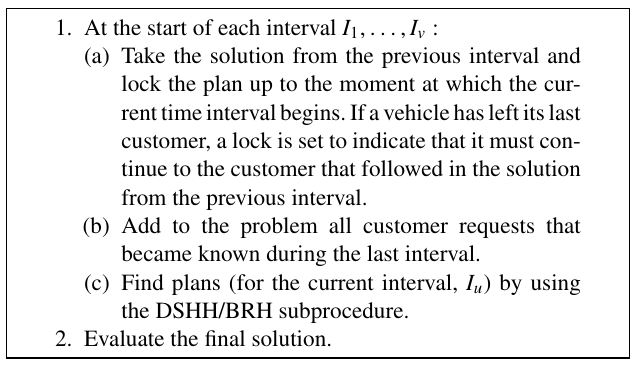
\includegraphics[width=0.5\textwidth,height=\textheight]{Images/OuterLoopBRH.png}
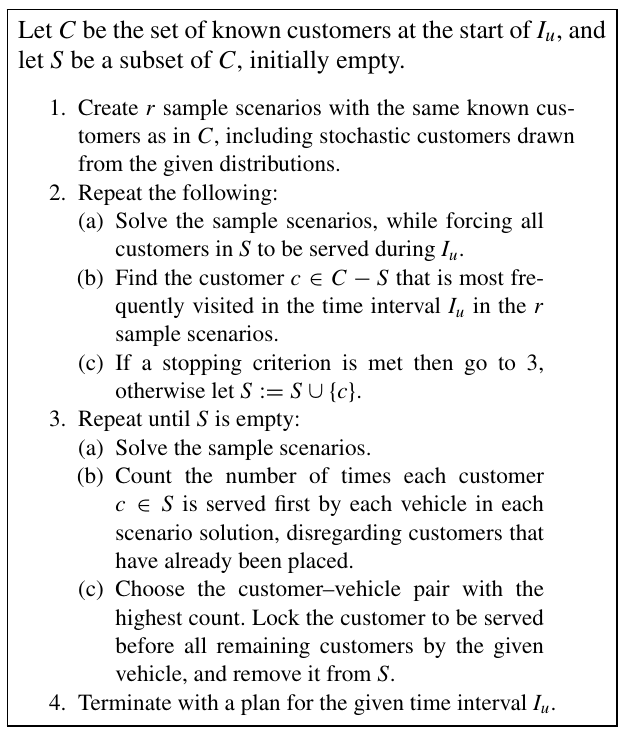
\includegraphics[width=0.49\textwidth,height=\textheight]{Images/InnerLoopDDSH.png}
    %\caption{Caption}
    %\label{fig:my_label}
\end{figure}



L'immagine a destra mostra il ciclo interno dell'euristica
{\(\mathbf{DSHH}\)} che usa l'informazione riguardo agli eventi futuri
per costruire \textbf{scenari campione}, una volta che viene fissato
l'intervallo corrente nel loop esterno descritto dall'immagine a
sinistra. Uno scenario campione è interpretato come una possibile
realizzazione di eventi futuri ed infatti vengono generati usando
distribuzioni di probabilità che si suppongono essere ottenute da dati
passati. L'euristica Branch-and Regret {\(\mathbf{BRH}\)} ha lo stesso
loop esterno che gestisce l'aspetto dinamico del problema, ossia fissa
in soluzione tutta la parte di piano dell'intervallo precedente che è
stata eseguita. Le due euristiche si differenziano per il loop interno e
quindi nel modo in cui vengono determinati i percorsi per i veicoli
usando gli scenari campione che includono sia tutta l'informazione certa
disponibile all'iterazione corrente sia l'informazione stocastica
campionata. In entrambe le euristiche questa sotto procedura viene vista
come composta di due fasi:

\begin{enumerate}
\tightlist
\item
  la prima in cui viene scelto iterativamente l'insieme dei clienti da
  gestire nell'intervallo corrente, usando come criterio di selezione la
  frequenza della loro presenza all'interno delle soluzioni degli
  {\(r\)} scenari generati. Il processo di selezione dei clienti
  continua fino a quando non vi sono in nell'insieme {\(S\)} dei clienti
  da servire una buona proporzione dei clienti serviti dalla maggioranza
  degli scenari. Questa proporzione rappresenta quindi il criterio di
  arresto e i clienti dovrebbero continuare a essere scelti fintanto che
  sono serviti in non meno della metà delle soluzioni di scenario di
  esempio;
\item
  nella seconda fase si pianifica il routing e viene iterativamente
  fissato nel piano il cliente (con associato il veicolo) che viene più
  frequentemente servito per primo all'interno degli scenari generati.
  Una volta fissato un cliente, viene tolto dall'insieme {\(S\)} delle
  richieste da pianificare e si ripete il passo fino a che ogni cliente
  in {\(S\)} non ha una posizione nella sequenza delle richieste da
  gestire. Possiamo notare come questa seconda fase consista di due
  decisioni separate: quale veicolo usare per un cliente e in quale
  ordine ogni veicolo deve gestire le richieste che gli sono state
  associate.
\end{enumerate}

Un aspetto negativo dell'euristica {\(\mathbf{DSHH}\)} è che
occasionalmente prevede di usare più veicoli di un approccio miope che
non usa l'informazione stocastica. Una possibile spiegazione di questo è
che sebbene selezionare un cliente gestito dal maggior numero di scenari
sia un criterio più che ragionevole, può capitare che venga gestito
differentemente da un minor numero di scenari per una valida ragione,
come ad esempio la necessità di veicoli aggiuntivi in futuro.
Presentiamo la {\(\mathbf{BRH}\)}:

\begin{figure}
    \centering
    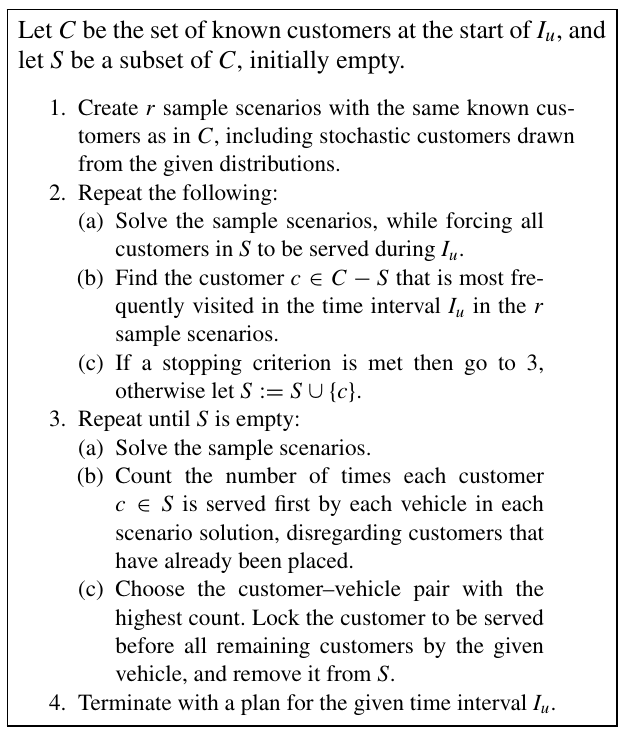
\includegraphics[width=0.6\textwidth,height=\textheight]{Images/InnerLoopDDSH.png}
    %\caption{Caption}
    %\label{fig:my_label}
\end{figure}

La {\(\mathbf{BRH}\)} cerca di correggere questo comportamento della
{\(\mathbf{DSHH}\)} andando a valutare le decisioni selezionate in base
ai conteggi delle frequenze e a implementare solamente quelle che
evitano effetti negativi nella pianificazione complessiva. In ogni
iterazione dei loop {\(2.\)} e {\(3.\)}, in cui si generano scenari, la
{\(\mathbf{BRH}\)} si comporta in questo modo:

\begin{itemize}
\tightlist
\item
  produce le soluzioni di ogni scenario campione separatamente;
\item
  unisce le soluzioni usando criteri di branch che riguardano decisioni
  chiave effettuate;
\item
  seleziona solo uno dei branch generati in base alla valutazione
  ottenuta con un criterio di regret. Generalmente questo criterio si
  basa sulla bontà media delle soluzioni di tutti gli scenari campione
  una volta che viene fissata la decisione che contraddistingue il
  branch.
\end{itemize}

Per il ciclo {\(2.\)} la decisione ad esempio riguarda la scelta di
inserire {\(c\)} in {\(S_{IN}\)} o in {\(S_{OUT}\)}, mentre per il ciclo
{\(3.\)} riguarda la scelta della coppia cliente-veicolo da fissare.
Dato che il {\(\mathbf{BRH}\)} abbiamo la lista {\(S_{OUT}\)} dei
clienti da non gestire nell'iterazione corrente, il ciclo {\(2.\)} non
ha bisogno di un parametro per il criterio di terminazione, ma può
continuare fino a quando non è stata presa una decisione per tutti i
clienti.\\
Per la creazione delle soluzioni degli scenari campioni sia
{\(\mathbf{BRH}\)} che {\(\mathbf{DSHH}\)} prevedono un semplice
criterio: inziano con una route vuota e, visitando i clienti in ordine
randomico, gli inseriscono uno alla volta nella migliore posizione.

\hypertarget{mathbfbrh-per-lestensione-di-mathbfsdvrp}{%
\subsection{\texorpdfstring{BRH per l'estensione di
SDVRP}{BRH per l'estensione di SDVRP}}\label{mathbfbrh-per-lestensione-di-mathbfsdvrp}}

Introdurre la possibilità di avere richieste stocastiche per clienti
noti porta ad alcuni cambiamenti in {\(\mathbf{BRH}\)}.

\hypertarget{cambiamento-negli-scenari}{%
\subsubsection{Cambiamento negli
scenari}\label{cambiamento-negli-scenari}}

Un primo cambiamento riguarda la risoluzione degli scenari campione.
Nota infatti che data la stocasticità delle richieste questa può
assumere valori diversi in diversi scenari. Pertanto, quando si
producono le soluzioni agli scenari campione, si dovrebbero riflettere
le corrette azioni di ricorso, in modo che i clienti selezionati del
{\(\mathbf{BRH}\)} non debbano più essere necessariamente serviti
durante l'intervallo, sebbene debbano essere visitati. Pertanto, il
criterio di inserimento per la risoluzione degli scenari campione viene
leggermente modificato, in modo che se un cliente con domanda stocastica
viene selezionato per il servizio entro l'intervallo successivo, verrà
servito entro l'intervallo, se possibile, o altrimenti visitato e quindi
servito in seguito. Ciò si ottiene, in ogni scenario campione,
suddividendo il cliente selezionato in due parti: una parte che deve
essere visitata entro l'intervallo di tempo successivo e una parte che
rappresenta il ritiro, sebbene le due parti, se possibile, verranno
inserite in punti consecutivi nella tratta di un veicolo.

\hypertarget{ammissibilituxe0}{%
\subsubsection{Ammissibilità}\label{ammissibilituxe0}}

L'altra conseguenza di includere richieste stocastiche riguarda la
possibilità che qualche cliente non venga servito nonostante sia
conosciuto fin dall'inizio, a causa dei vincoli di capacità. Nonostante
questo non capiti sovente vi è la possibilità che nell'ultimo intervallo
di tempo, gli scenari campione falliscano nel rappresentare la richiesta
del cliente, sottostimandola, e che non venga quindi alla fine servito
perchè la sua richiesta reale viene scoperta solo alla fine. Per
prevenire questo, usufruendo del fatto che le finestre temporali di tali
clienti sono generalmente molto larghe e non problematiche, si può
forzare la visita di tali clienti prima dell'ultimo
intervallo.

\hypertarget{conclusioni}{%
\section{Conclusioni}\label{conclusioni}}

Questo paper estende il lavoro precedente degli autori in due direzioni:

\begin{itemize}
\tightlist
\item
  è stata migliorata la procedura di risoluzione euristica, consolidando
  il fatto che l'uso della conoscenza stocastica in problemi
  {\(\mathbf{VRP}\)} dinamici portano a migliori risultati, anche quando
  l'informazione è usata solamente per creare esempi di scenari;
\item
  è stato esteso il problema originale permettendo richieste stocastiche
  per clienti noti e mostrando come la nuova euristica permetta di
  ottenere buoni risultati seppur trattando diversi tipi di
  stocasticità.
\end{itemize}

\end{document}
